% 06.1.4. TAREAS Y ESTIMACIONES DE ESFUERZOS POR ITERACIÓN 
%----------------------------------------------------------------------------------------


\paragraph{} Se muestran los esfuerzos previstos para la primera iteración en la figura \ref{fig:6141}.

\begin{figure}[h!]
\centering
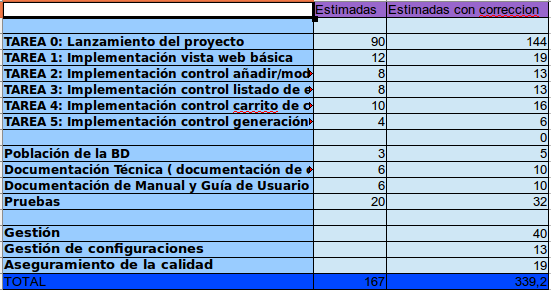
\includegraphics[width=0.95\textwidth]{img/6141}
\caption{Esfuerzos primera iteración}
 \label{fig:6141}
\end{figure}

\paragraph{} Se puede apreciar como la parte más importante de la primera iteración fue el lanzamiento, en el cual se planifico todo el proyecto para concretar todo e intentar evitar posibles problemas. Entre las demás partes se planifico que pruebas, gestión y implementación serías las siguientes tareas más costosas. Esto se puede ver en la~\cref{fig:6142}.

\begin{figure}[h!]
\centering
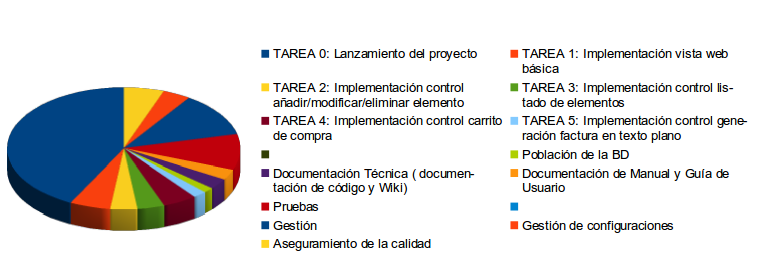
\includegraphics[width=0.95\textwidth]{img/6142}
\caption{Gráfica esfuerzos primera iteración}
 \label{fig:6142}
\end{figure}

\paragraph{} Se muestran los esfuerzos previstos para la segunda iteración en la~\cref{fig:6143}.

\begin{figure}[h!]
\centering
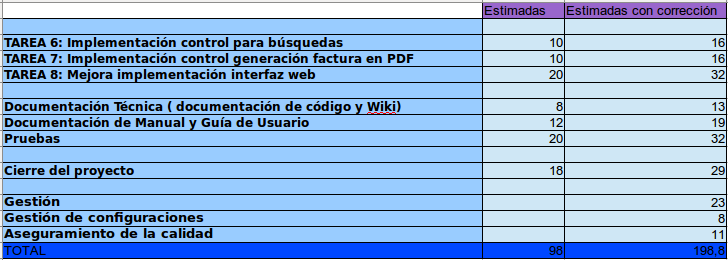
\includegraphics[width=0.95\textwidth]{img/6143}
\caption{Esfuerzos segunda iteración}
 \label{fig:6143}
\end{figure}

\paragraph{} En la segunda iteración se siguieron más o menos los patrones de la primera.

\begin{figure}[h!]
\centering
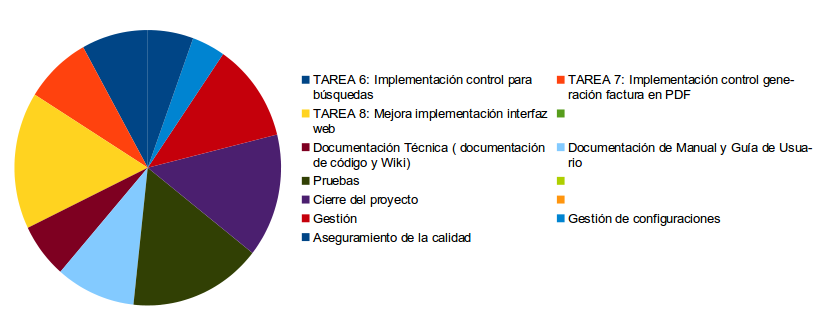
\includegraphics[width=0.95\textwidth]{img/6144}
\caption{Gráfica esfuerzos segunda iteración}
 \label{fig:6144}
\end{figure}